\newpage
\subsection{Befugter - Jens}
\subsubsection{Design}
For at opretholde et optimalt udrugningsmiljø, er det nødvendigt med befugtning af luften i rugemaskinen. Følgende afsnit vil omhandle dette emne.

Der har været følgende design idéer i spil:

\begin{itemize}
  \item  Dryppe vand direkte på varmelegeme, for derefter at lade varmelegemet fordampe vandet.
  \item Forstøvet vandet fint via en dysse.
\end{itemize}
 
Det blev valgt at gå videre med idéen om at forstøve vandet via en dysse.
 Første udkast bestod i:
\begin{itemize}
	\item En beholder fyldt med vand under et konstant tryk via en kompressor, selve styringen af forstøvningen af vandet skulle forgå ved at åben/lukke en magnetventil.
\end{itemize} 
Denne idé blev droppet da det ville kræve at brugerne af rugemaskinen skulle have adgang til en kompressor, samt der skulle bestilles en typegodkendt trykluftbeholder hjem, hvilket ville forøge udgifterne til projektet væsentligt.
\subsubsection{Implementering}

Nedenstående figur \ref{fig:Havesprojte_implement_rapport} illustrerer den færdige implementering af hardware delen til befugtning af luften. 

\begin{figure}[H]
\centering
{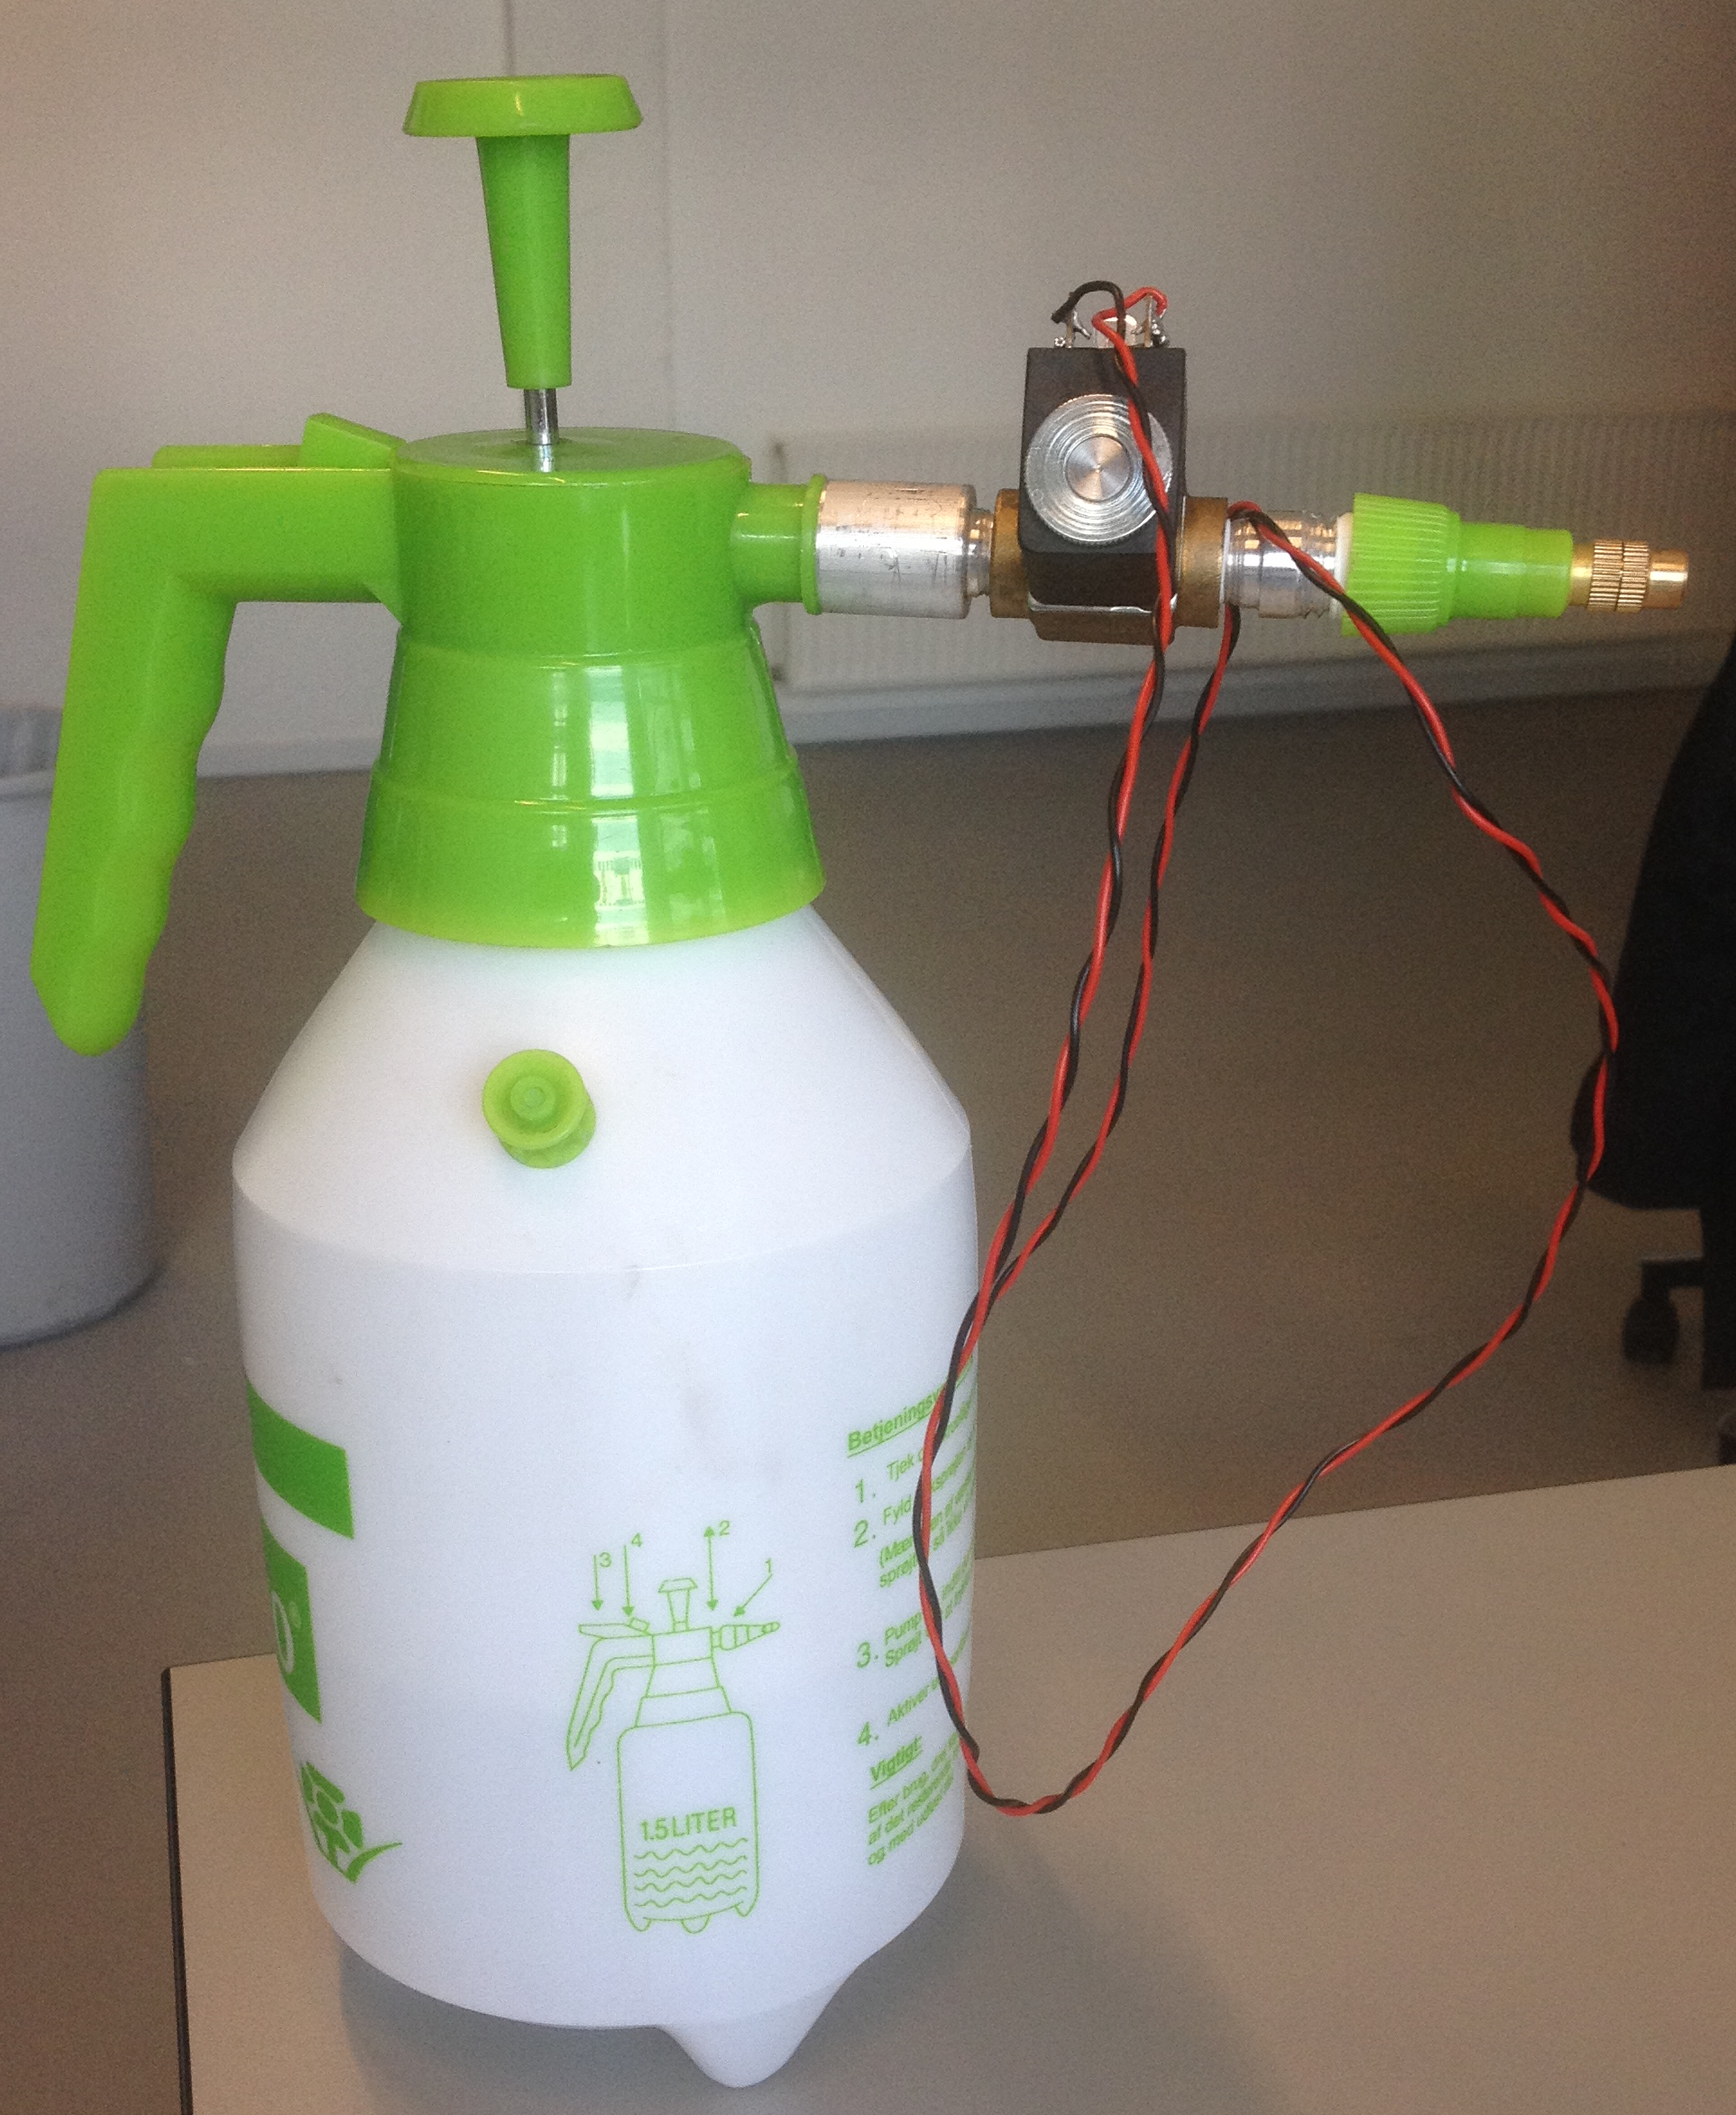
\includegraphics[page=1,scale=0.08,trim=5mm 5mm 5mm 5mm]{./7_projektbeskrivelse/design_og_implementering/hardware/havesprojte_implemt.png}}
\caption[Figur]{Havesprøjte med på monteret magnetventil}
\label{fig:Havesprojte_implement_rapport}
\end{figure}

Via en empirisk tilgang blev der fundet frem til at den korteste puls der kunne åbens for befugtningen med var 10ms. Denne tilgang bestod i at skrive et test program til PSoC3 til aktiveringen af magnetventilen, hvor det gradvist blev prøvet at sænke varigheden på åbnings impulsen. 
\begin{itemize}
\item 5ms var ikke nok til at magnetventil kunne nå at åben.
\item 7ms var lige grænsen for hvad der kunne lande sig gøre, da dette gav et udstabilt resultat 
\end{itemize}